\chapter[Perception of melodic detail]{Perception of melodic detail}\label{sec3}
In the previous chapter we documented regularities in speakers' productions which are not accounted for by the Autosegmental-Metrical (AM) model of intonational phonology. Moreover, it appears that this previously unacknowledged phonetic information allows for the elaboration of metrics which are more effective than traditional AM indices in mirroring some pragmatic contrasts. However, regularity in production and robust mirroring of pragmatic contrasts are not sufficient reasons to motivate the inclusion of phonetic information into phonological representations. The additional requirement to be met is actual use of this phonetic information in perception. If phonetic information is regularly produced but not exploited in perception (or, more radically, not perceived at all), then it could be deemed a by-product of other contrasts, and its inclusion in a minimalist phonological representation would not be justified. As we saw in  Section~\ref{sec242}, enriching phonological representations is a complex operation. For this reason, before prospecting any modification in the inventory or in the grammar of the intonational phonology of Neapolitan Italian (NI), an evaluation of the perceptual role of the regularities found in production is in order.

\section{Introduction}\label{sec31}
Even if perception of intonation has witnessed a growing interest from the research community since the 1960s, few are the studies which concentrate on the perception of phonologically salient dynamic proprieties of \textit{f0} contours.\is{f0 dynamics} Such studies seem to bring together the two main threads which characterized research on intonation perception, and which can also be (although very loosely) diacronically arranged. Early studies focussed on the psychoacoustics of pitch perception, in the attempt of defining how listeners deal with fundamental frequency modulations over time (at least since \citealt{sergeant1962sensitivity}). This research agenda, combined with the relative unavailability of stable procedures for speech resynthesis,\footnote{Linear Predictive Coding (\textit{LPC}) based resynthesis was only available in 1970s, while Pitch-Synchronous OverLapp-Add (\textit{PSOLA}) based methods are even more recent.} motivates at least partially the pervasive use of simple non-speech signals as the basis for stimuli construction.\is{resynthesis} However, it soon became evident that the pure tones used in early psychoacoustically-oriented research were but a first step towards the study of the specificities of the speech signal. The use of speech-like material in pitch perception investigations \citep{rossi1971seuil,klatt1973discrimination,thart1976psychoacoustic,schouten1985identification} was instrumental in orienting research on the relationships between spectral content and \textit{f0} variation \citep{house1990tonal,house1997perceptual}, permitting a shift from psychoacoustic to properly linguistic research.

While the psychoacoustic approach was yielding its first mature fruits, research on the structure of intonational categories moved its first steps. A new look at intonation perception came from studies on categorical perception of segmental contrasts (see Section~\ref{sec111}): the exploration of the viability of the categorical perception \citep{kohler1987categorical} for intonation as well started a line of studies in which intonational categories are central. Different paradigms for exploring the warping of perceptual space in intonation were proposed and tested, from classification and discrimination to imitation \citep{pierrehumbert1989categories}, semantic differential (from  \citealt{osgood1957measurement} through \citealt{uldall1964dimensions} to \citealt{kirsner1994interaction}) and indirect identification (context matching, \citealt{nash1980intonation}), up to eye-tracking \citep{dahan2002accent}. It seems that, unlike the one focussing on the pychoacoustics of pitch perception, this research thread on intonational categories still draws linguists' attention, as recent work questioning the viability of categorical perception for intonation \citep{gussenhoven2006experimental,niebuhr2007categorical} shows.

Studies on the role of dynamic \textit{f0} contour cues in perception bring together these two lines of research, in that they rest at the same time on a deep understanding of how much detail in the signal is psychoacoustically perceptible and of how intonational categories can be identified.

\subsection{Perception of melodic detail}\label{sec311}
In this section we will review two such studies, dealing respectively with NI \citep{petrone2011tones} and with Northern Standard German \citep{petrone2014intonation}. Both studies analyze prenuclear falls and show that sentence modality contrasts are not exclusively cued by the intonational nucleus.\is{sentence modality} 

The first builds on production results of \citet[see Section~\ref{sec241}]{petrone2008tonal}\is{Neapolitan Italian}, in which the authors accounted for different shapes in prenuclear falls by suggesting a tonal contrast (H in questions and L in statements) for the tone associated to the right edge of the Accentual Phrase domain. A subsequent study \citep{petrone2011tones} then tests with two experiments the perceptual role of the Accentual Phrase tone, under the hypothesis that listeners do not rely exclusively on nuclear pitch accent contrasts in order to classify questions and statements. The first experiment is based on an identification task using gated stimuli (see Figure~\ref{fig301}). Utterances are cut after the prenuclear pitch accent (PREN condition) and after the alleged Accentual Phrase tone (AP condition), and they were presented to listeners along with control uncut stimuli (NUCL condition) for classification as either Statements or Questions. 

\begin{figure}
\centering
\resizebox{\linewidth}{!}{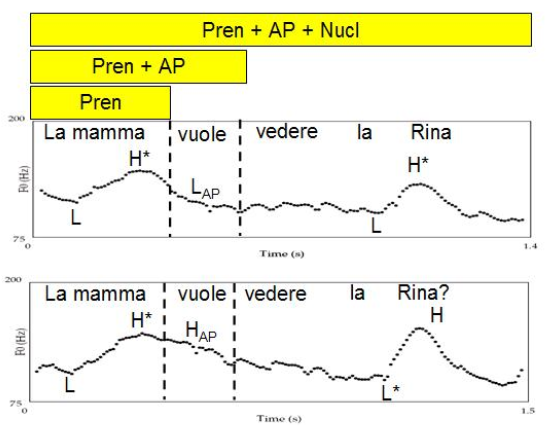
\includegraphics{images/301.png}}
\caption{Schematized representation of the stimulus manipulation (three conditions: PREN, AP, NUCL) for the sentence \textit{La mamma vuole vedere la Rina}, uttered as a narrow focus statement with late focus (upper picture), and as a yes/no question (lower picture). From Petrone and D'Imperio (2011), original caption.}
\label{fig301}\end{figure}

Results show that classification scores are already above chance level for the PREN condition, and that in AP condition classification is even more robust for statements, but not for questions.\footnote{This latter finding is the starting point for the second experiment, in which a semantic differential task is used to assess the nature of the meaning (attitudinal or pragmatic) conveyed by the AP tone.} The authors suggest that the absence of a significant improvement in question identification from the PREN to the AP condition could be due to the fact that the \textit{f0} contour stretching from the prenuclear peak to the H Accentual Phrase tone has a characteristically concave shape if compared to the convex shape of the interpolation between the peak and the L Accentual Phrase in statements. If listeners relied on this difference in \textit{f0} contours to classify stimuli, the same performances would indeed be expected for PREN and AP condition. It is interesting to note that a difference in the shape of the fall, described with different tonal specifications for the AP right edge, actually seems to be perceived even in stimuli gated before the AP itself. In a radical perspective, this finding could be taken as evidence against the adequacy of a representation based on AP tones, and rather supporting the hypothesis that the shape of the interpolation between tonal targets is relevant in itself: in the concluding remarks, the authors themselves acknowledge the need for a closer examination of dynamic proprieties of the fall.

The perceptual role of prenuclear falls has been investigated for Northern Standard German as well \citep{petrone2014intonation}.\is{German} In their first experiment, syntactically declarative Subject-Verb-Object sentences were uttered as questions or statements, using different nuclear configurations: statements all had a L- L\% utterance-final fall combined with one of three different pitch accents (H+L*, H* and L*+H in AM terms or early, medial and late peak in KIM terms; see Section~\ref{sec242}); questions had an L*+H pitch accent combined with either a final fall (L- L\%) or rise (H- H\%). The working-hypothesis transcription for the prenuclear fall was H*, but some phonetic differences between questions and statements could be spotted in the slope and the shape of the fall (see Figure~\ref{fig302}).

\begin{figure}
\centering
\resizebox{\linewidth}{!}{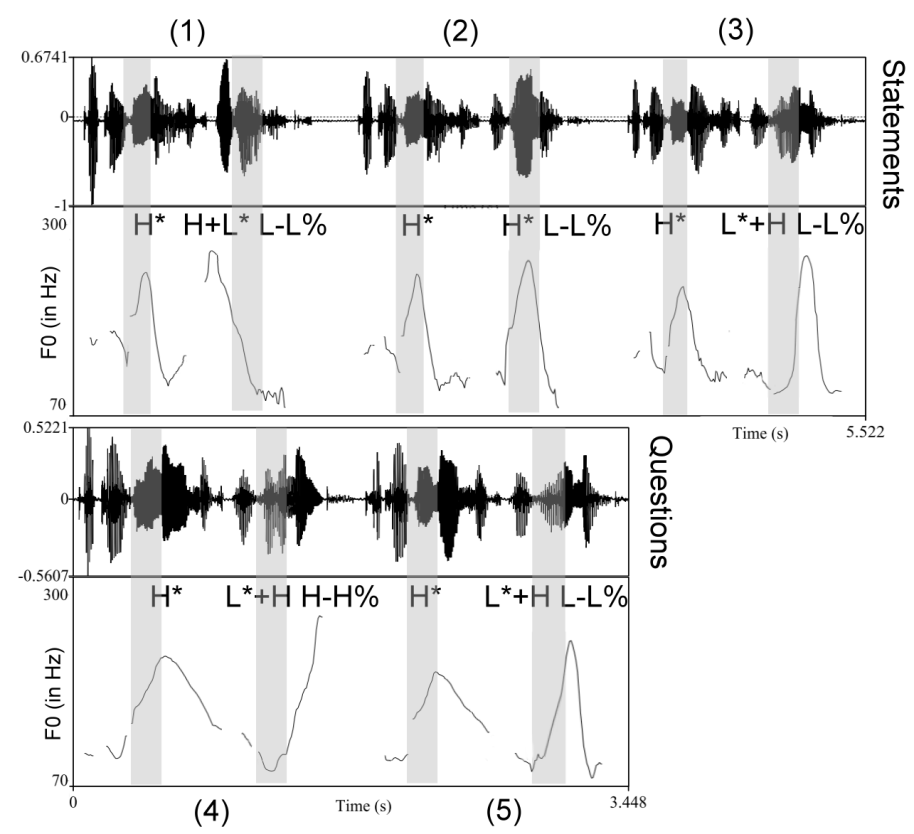
\includegraphics{images/302.png}}
\caption{Oscillograms, \textit{f0} contours (70-300 Hz) and corresponding phonological analyses of the five naturally produced stimuli \textit{Katherina sucht 'ne Wohnung}; (1)-(3) were produced as statements, (4)-(5) were produced as questions. The syllables \textit{-ri-} and \textit{Woh-} that showed the prenuclear and nuclear accents are highlighted in grey. From Petrone and Niebuhr (2014), original caption.}
\label{fig302}\end{figure}

Natural utterances were gated at after the Subject and the Verb and presented (along with control uncut items) to listeners for a semantic differential task on three scales, namely astonishment, uncertainty and questioningness. Results show that phonetic information in prenuclear falls is actually used by listeners in order to classify questions and statements: original questions sound more astonished, uncertain and questioning than original statements, even when gated right after the Subject, that is before the nuclear configuration. This is not to say that the nucleus itself plays no role: complete utterances yield stronger responses towards the astonished, uncertain and questioning pole of the semantic scales.\footnote{The increase is maximal when compared with stimuli gated after the Verb. For these cases, the authors suggest a Frequency Code based explanation for listeners' bias towards statement-like responses, given that \textit{f0} on the Verb is a low plateau. However, a syntax based bias could also contribute to this result.} This finding leads the authors to claim that phonetic detail in \textit{f0} contours can even be spotted in the nuclear pitch accent labelled as L*+H, which would have a more convex rise in statements and a more concave rise in questions. However, this evidence is not compelling, since the availability to the listener of a L*+H pitch accent seem to induce more question-like responses for original statements as well.

The second experiment aimed at precisely identifying which of the melodic properties in the prenuclear region are actually responsible for the shift in listeners' perception. Stimuli with resynthesized peak alignment, fall slope and fall shape in the prenuclear region were used in a context matching task. Results show that alignment, slope and shape interact in cueing sentence modality: question classification, for example, is strongest with early aligned peak, shallow fall slopes and concave shapes. On the basis of this evidence and of the similar findings reported by \citet{petrone2011tones} for NI, the authors underline the necessity of accounting for \textit{f0} dynamic information in phonological representations of prenuclear regions in German, through a different specification of either the prenuclear pitch accents (to be differentiated via trailing tones) or an alleged edge tone of a new prosodic domain (as in the NI analysis).

The two studies we reviewed in this section are both concerned with the prenuclear region, where shape differences can be attributed to either pitch accents or edge tones, as we have seen in the discussion of the German data. In the following section, building on previous work \citep{dimperio2009interplay}, we report on two experiments on the perception of the nuclear rise shape differences we documented in Section~\ref{sec2}.\is{pitch accent} Focussing on nuclear rises has the advantage of discarding any account of shape differences based on additional edge tones, thus enabling a more straightforward phonological modelling of the data. Both experiments (henceforth E1 and E2) are based on a categorization task and use stimuli resynthesized from utterances contained in the \textit{Tre Grazie} corpus (see Section~\ref{sec221}).

\section{Experiment 1}\label{sec32}
\subsection{Background}\label{sec3200}
The general aim of E1 was to test whether pitch accent classification is affected by dynamic intonational cues.\is{f0 dynamics} Specifically, building on the regularities found in speakers' productions (see Section~\ref{sec2}), we tested the perceptual role of rise shape in the contrast between nuclear accents of partial topic statements (SPT)\is{partial topic} and narrow focus questions (QNF).\is{narrow focus} If rise shape differences are consistently produced by speakers and reliably used by listeners, then phonological representations of pitch accents should indeed include this phonetic information: rise shape would qualify as prosodic detail in the sense of useful information not yet encoded in abstract accounts of intonation. In order to test this hypothesis, we devised a forced-choice categorization task in which we manipulated rise shape (from concave to convex), asking subjects to classify items as questions or statements. If listeners use rise shape information in classification, we expect more question responses for stimuli with a more convex rise and more statement responses for stimuli with a more concave rise.

In addition to rise shape, we decided to test the impact of another cue, namely the scaling of the elbow following the peak in the stressed syllable.\footnote{L1 alignment, in addition, was manipulated in order to test whether the entire rise is aligned later in questions; see \citet{dimperio2003tonal}. Since this issue is not relevant here, we will not comment it any further.\label{footnoteL1}} As we discussed in Section~\ref{sec241}, \citet{petrone2008tonal} showed that productions of focus-final statements and questions in NI are characterized by postnuclear falls having different shapes, namely more concave in questions and more convex in statements. They suggested that this contrast can be accounted for by a different tonal specification of a new prosodic domain, the Accentual Phrase, which would bear a H tone in questions (hence the concave fall) and a L tone in statements (hence the convex fall). Our corpus, on the other hand, focussed on shape differences in nuclear rises, and moreover on a different pragmatic contrast, namely the one between partial topic statements and narrow focus questions. However, through an examination of the \textit{Tre Grazie} corpus, \citet{dimperio2011phrasing} show that shape can also vary in postnuclear falls, with Partial Topics being characterized by an intermediate shape between concave questions and convex statements. In \citeauthor{petrone2008tonal}'s \citeyearpar{petrone2008tonal} terms, SPT would also have an Accentual Phrase break, whose tonal specification could be transcribed as !H in order to account for the three way contrast with statements (L) and questions (H). Independently of the phonological analysis, it is true that at least in some cases postnuclear falls present different shapes in SPT and QNF, as Figure~\ref{fig201} also shows. For this reason, in the design of our perception experiment we decided to add the fall shape factor along with the rise shape we already discussed above. In order to be able to tell apart the contribution of these two factors, we tested them both individually and jointly, thus creating three different manipulation sets (rise, fall, both rise and fall).

\subsection{Hypotheses}\label{sec320}
E1 allows us to test two hypotheses concerning the classification as narrow focus questions or partial topic statements of trisyllabic stimuli bearing a nuclear accent:

\begin{description}
   \item[H1:] \textit{identification is affected by rise shape}. The production experiment reported in Section~\ref{sec2} showed different interpolation forms between the tonal targets composing a rising accent. According to the null hypothesis, these differences are to be considered redundant phonetic information. The alternative hypothesis is that rise shape is perceptible and indeed used in classification.
   \item[H2:] \textit{identification is affected by fall shape}. Production data on prenuclear accents indicate that questions and statements are characterized by different fall shapes. According to the null hypothesis, these findings can not be extended to nuclear accents.
\end{description}

Given current limitations in our understanding of trading relationships between supposed phonetic details on different dimensions, we will restrain from explicitly formulating hypotheses on the joint manipulation of rise and fall.

Support for the alternative hypotheses will be evaluated by fitting subjects' responses to a Logit Mixed Model and by gauging the statistical significance of the factor \textit{Stimulus step} (from allegedly SPT-like to QNF-like) for each of the two manipulation sets, namely rise shape (for H1) and fall shape (or scaling of the postaccentual elbow for H2). Significance level was set to $<$ 0.05.

\subsection{Method}\label{sec321}
The first forced-choice categorization task involved 22 native speakers of NI, mainly undergraduate science students with no training in linguistics. The experiment took place in a silent room, using a personal computer and a professional headphone set.\footnote{We would like to thank Franco Cutugno for allowing us to use the facilities at \textit{DSFMN} (Dipartimento di Scienze Fisiche, Matematiche e Naturali), Naples University ``Federico II'', as well as Bogdan Ludusan for his assistance.} Subjects listened to audio stimuli and had to identify them as either Questions or Statements. They were asked to put their index fingers in resting position above one of the two designated computer keys, each bearing a coloured sticker label (blue on far left of the keyboard, red on the right). The colour code was reminded throughout the whole experiment by on-screen instructions associating colours to the labels \textit{Domanda} (``Question'') and \textit{Risposta} (``Answer''), and was counterbalanced across speakers. Stimulus presentation and response recording were managed by the software \textit{Perceval} \citep{andre2003perceval}. The task lasted about 30 minutes; subjects were allowed to take a break between any of the five blocks.

Each block was composed of 28 experimental resynthesized items and 18 control natural items. As control items we used 2 repetitions of the first word from 9 utterances in the \textit{Tre Grazie} corpus, recorded by a single speaker. Two SPT and two QNF utterances of the two sentences \textit{Valeria viene alle nove} and \textit{Amelia dorme da nonna} were cut after the Subject, yielding 8 of the control items.\footnote{See Section~\ref{sec221} for more details on the test sentences (6-8) and the pragmatic contexts (9-10).} The ninth control item also served as the starting point for resynthesizing experimental items, and consisted in the first word of the sentence \textit{Milena lo vuole amaro}, uttered as a SPT. The control items, along with the full utterances they were extracted from, were used in the training phase to make sure that subjects understood the task and the labels employed. This was particularly important, since SPT utterances are not as prototypical of the Statement category as QNF utterances are of the Question category (see Section~\ref{sec323}). Control natural items were also used to determine a baseline for correct classification of resynthesized items (see Section~\ref{sec322}). 

Experimental stimuli were built by modifying the melodic properties of the base natural stimulus described above (\textit{Milena} as SPT) using the \textit{PSOLA} algorithm \citep{moulines1990pitchsyncronous} embedded in \textit{Praat} \citep{boersma2008praat}.\is{resynthesis} The first manipulation consisted in resynthesizing a base experimental stimulus with ambiguous \textit{f0} features between those of a SPT and a QNF (see Figure~\ref{fig303}, solid line). In order to do so, for the base natural stimulus we calculated values for scaling and alignment with respect to the stressed vowel’s boundaries of the \textit{f0} peak (H) and the inflection points on its left (L1) and its right (L2) (see Figure~\ref{fig303}, dotted line). Then we averaged these values with the ones extracted from a QNF utterance of the same speaker for the same sentence (see Figure~\ref{fig303}, dashed line). 

\begin{figure}
\centering
\resizebox{\linewidth}{!}{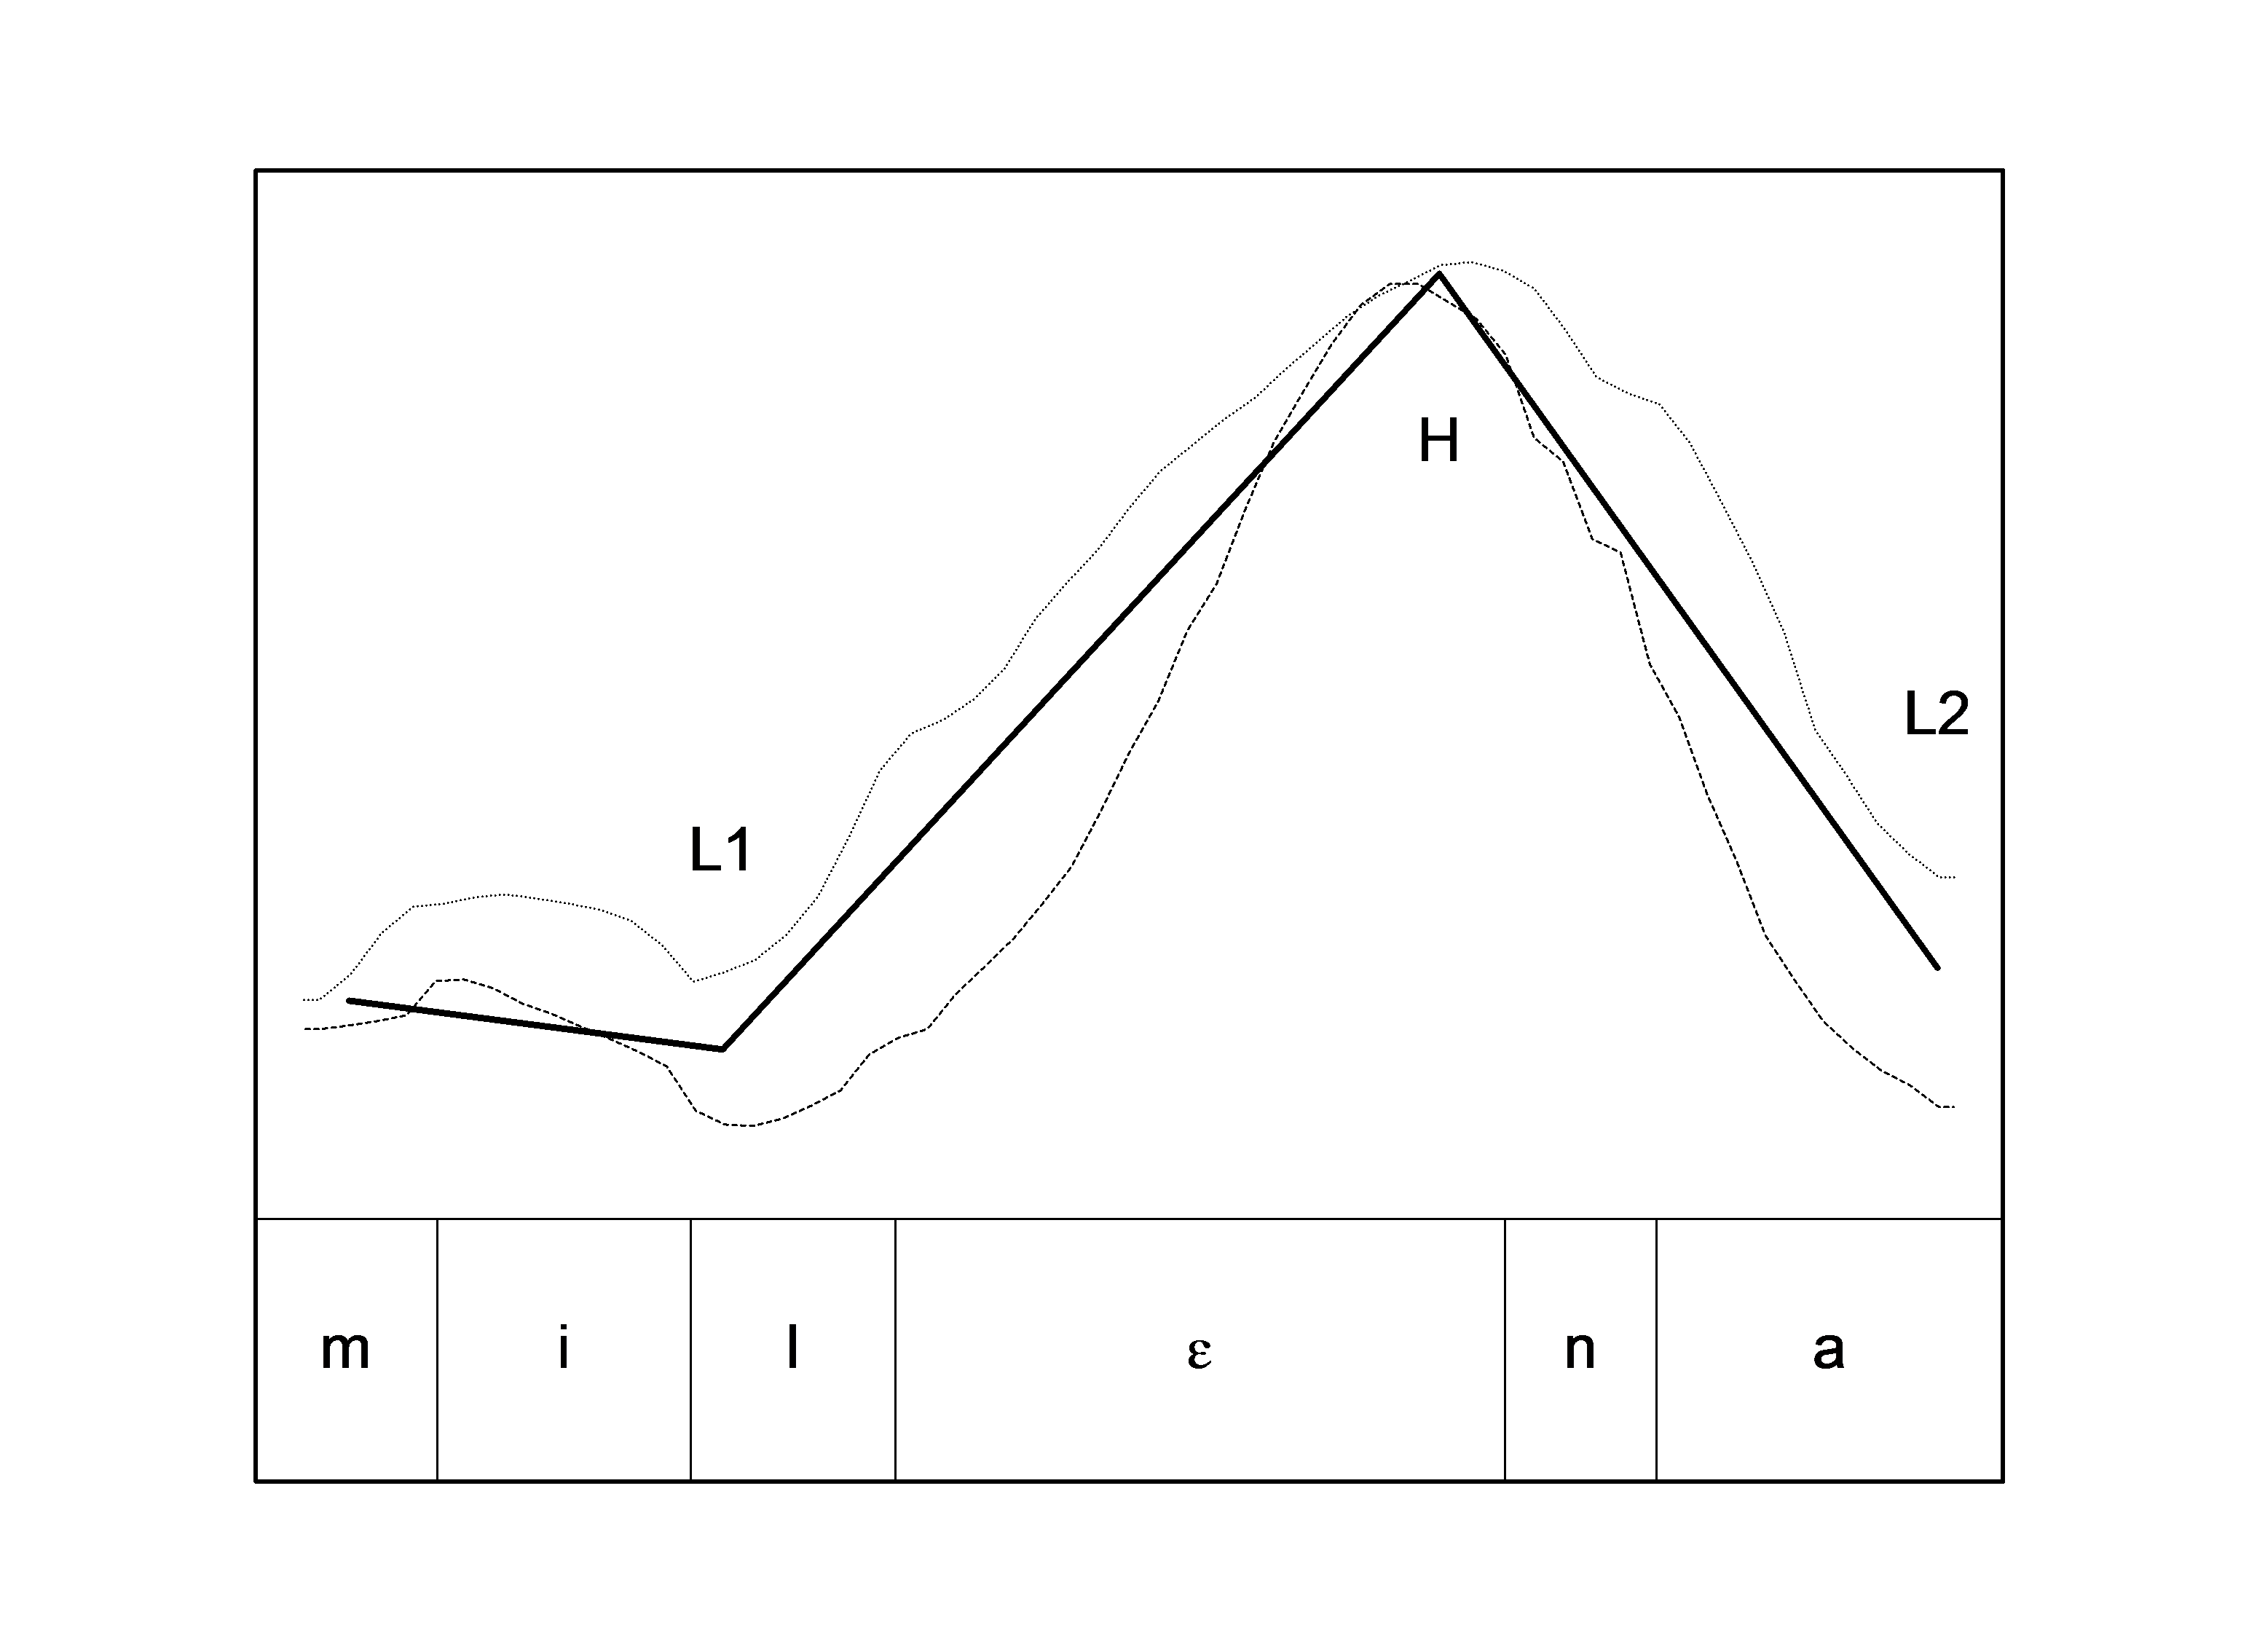
\includegraphics{images/303.png}}
\caption{Base stimulus averaging.}
\label{fig303}\end{figure}

The resulting stimulus was used as the starting point for further \textit{f0} manipulations. Four sets of stimuli were created by manipulating three dimensions and one of their combinations (see Figure~\ref{fig304} and Table~\ref{tab31}). The three dimensions were L1 alignment, rise shape and L2 scaling; the fourth set combined rise shape and L2 scaling manipulation. Each of the 4 sets was composed by 7 steps which were equally spaced in frequency as expressed in Hz.\footnote{In the first set (which we will not discuss any further; see Footnote~\ref{footnoteL1}) we manipulated L1 alignment, so steps were rather equally spaced in time.} Values of the ambiguous base stimulus were assigned to the central step (n. 4); values of the original stimuli were assigned to penultimate steps in the two directions (i.e. SPT = 2 and QNF = 6). This allowed us to create 4 sets which, for each parameter, went from an overtly SPT characterized stimulus (n. 1) to an overt QNF (n. 7). 

\begin{figure}
\centering
\resizebox{\linewidth}{!}{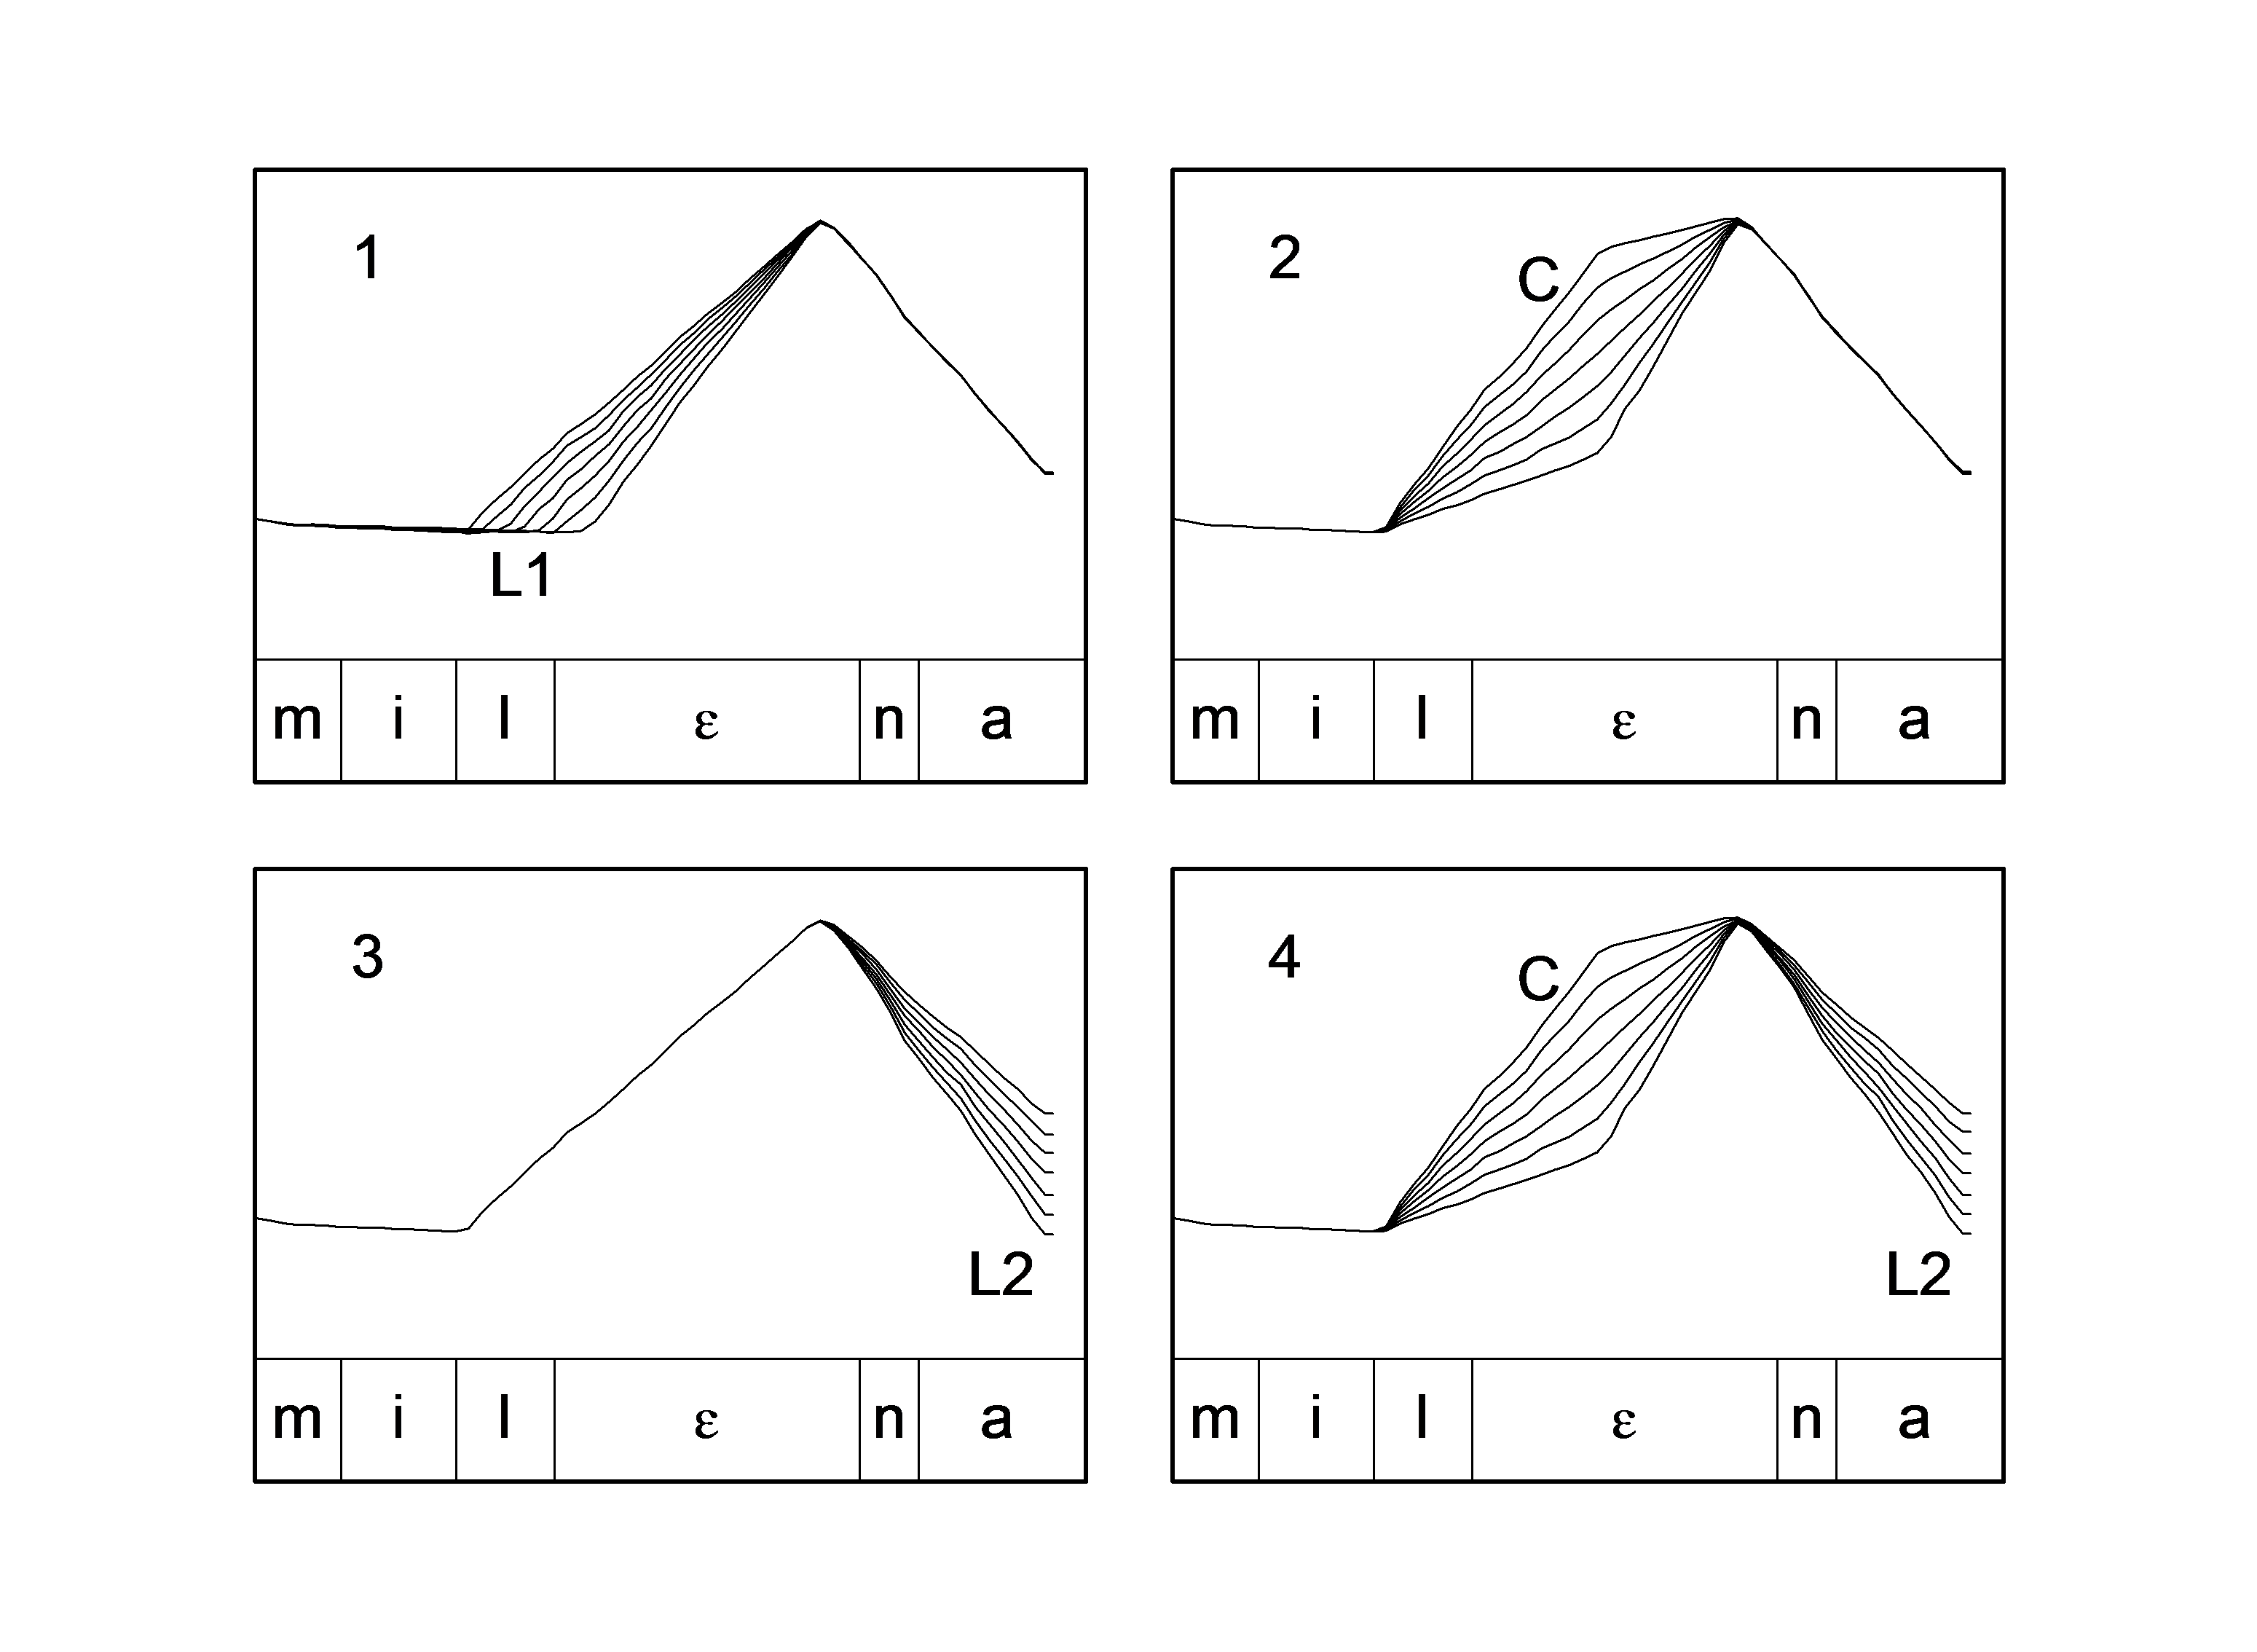
\includegraphics{images/304.png}}
\caption{Sketches of the 4 manipulation sets (1: L1 alignment; 2: rise shape; 3: L2 scaling; 4: rise shape and L2 scaling), aligned with the name \textit{Milena}.}
\label{fig304}\end{figure}

\begin{table}[h]
\centering
\begin{tabular}{c c c}
\mytoprule
Set & Feature(s) & Steps \\
\midrule
1 & L1 alignment & 15 ms \\
2 & Rise midpoint & 15 Hz \\
3 & L2 scaling & 10 Hz \\
4 & Rise midpoint and L2 scaling & 15 and 10 Hz \\
\end{tabular}
\caption{Summary of manipulations}
\label{tab31}\end{table}

We gathered 3080 responses for experimental items (22 subjects x 5 blocks x 4 sets x 7 steps) and 1980 for control items (22 subjects x 5 blocks x 2 repetitions x 9 stimuli).

\subsection{Results}\label{sec322}
Responses to control stimuli show that listeners found the task very difficult. During the training phase, no subject experienced difficulties in classifying the uncut stimuli. However, during the test phase, subjects had to classify 90 (5 blocks x 9 items x 2 repetitions) natural stimuli cut after the first word. Results show that only 5 out of 22 listeners managed to make a somehow reliable distinction (above 60\% of correct classification) between unresynthesized SPTs and QNFs.

Figure~\ref{fig305} (left panel) plots the frequency of Statement responses (y-axis) against the seven manipulation steps (x-axis) for the three individual sets (rise curvature, L2 scaling, rise curvature and L2 scaling), pooled across all subjects. The results do not show the expected trend to higher Statement responses for the first (1-3) manipulation steps. 

\begin{figure}
\centering
\resizebox{\linewidth}{!}{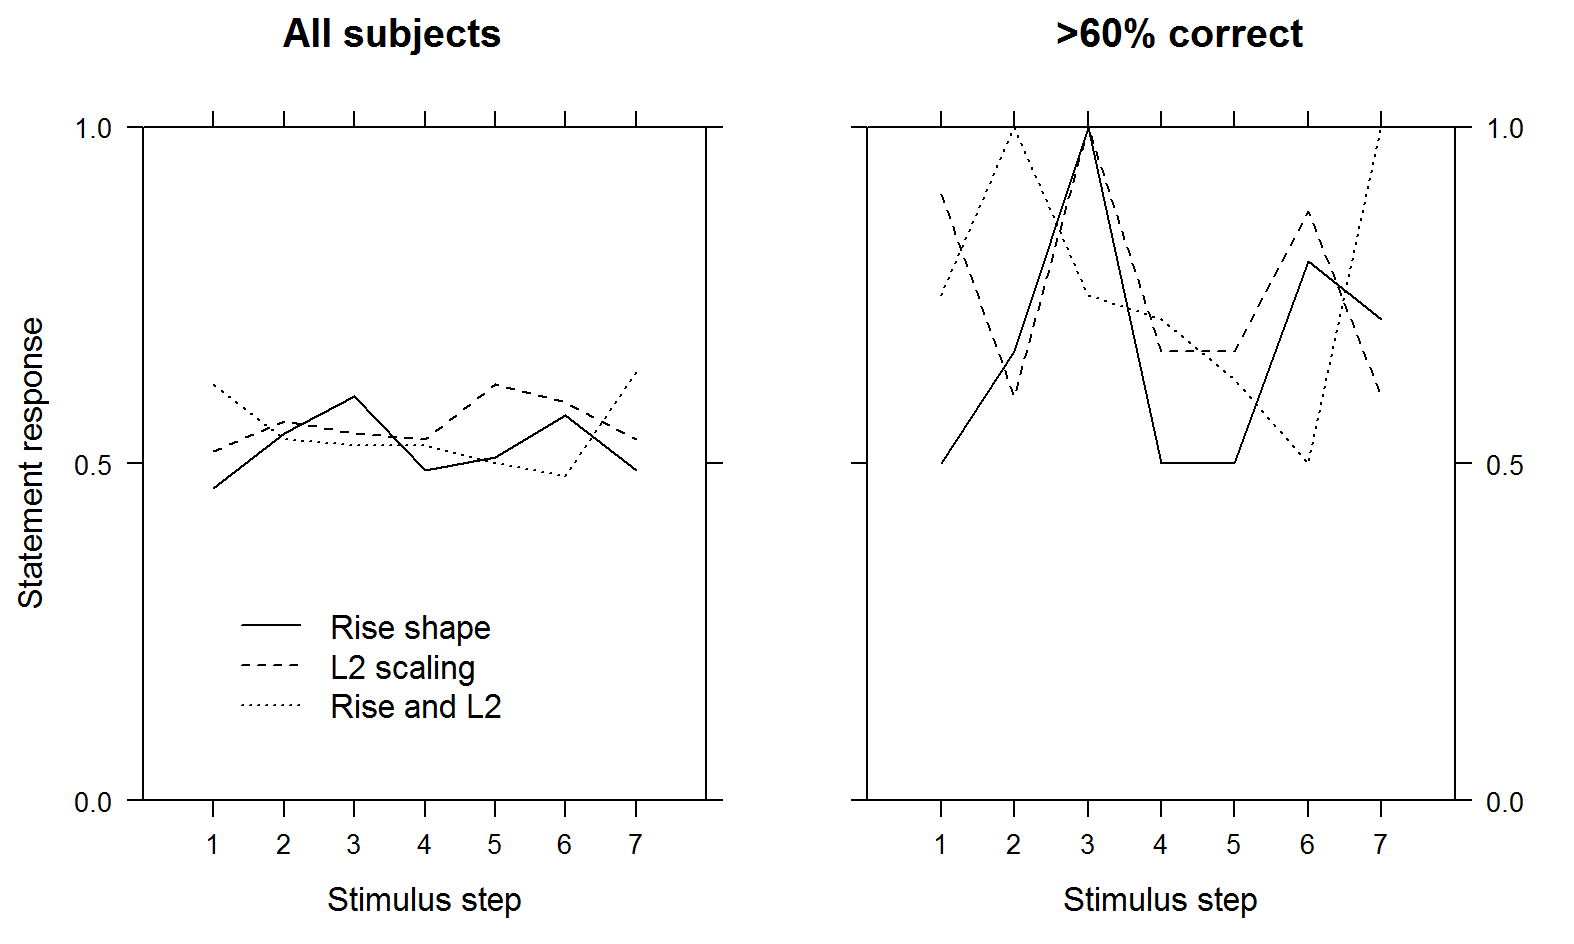
\includegraphics{images/305.png}}
\caption{Experiment I. Frequency of Statement responses for the three relevant manipulations sets (2-4 in Table 3.1). Data for all subjects (left panel) and for the 5 subjects with best performance on control items (right panel).}
\label{fig305}\end{figure}

Given the results of control items classification, we decided to plot separately the responses to experimental stimuli for the five subjects with the highest control performance, in order to ascertain whether the degree of sensitivity to resynthesis was different across subjects. However, as Figure~\ref{fig305} (right panel) shows, no trends are discernible for this subgroup either. Statistical analyses are omitted, since the visual inspection of the results clearly indicates no effect of any of the experimental treatments on subjects' responses, for both groups of subjects. The inspection of the two panels in Figure~\ref{fig305}, however, shows that the five ``reliable'' subjects had a slight bias towards the Statement response, irrespective of the dimension, the direction and the intensity of the manipulation (see Section~\ref{sec33} for discussion).

\subsection{Discussion}\label{sec323}
Results show that subjects do not use L1 alignment, rise shape or L2 scaling as cues for the classification of trisyllabic stimuli as narrow focus questions or partial topic statements. The interpretation of negative results being an epistemologically complex operation, in the following we will concentrate on some hypotheses accounting for this outcome, and on further testing needed in order to validate them.

First of all, it is possible that our manipulations did not involve phonetic information actually used in classification. In this case, the differences in rise shape we found to be consistent in production (see Section~\ref{sec2}) could be deemed perceptually irrelevant by-products of other paradigmatic options, as the tonal specification of the accentual phrase \citep{petrone2008tonal} or the compression of postnuclear register \citep{dimperio2011phrasing}. This perspective would constitute evidence for the appropriateness of a strongly abstractionist approach to intonation, in which some of the phonetic information contained in the signal, even if consistently present, is actually discarded in the mapping phase.

More radically, we could also hypothesize that our manipulations are not only unused in classification, but are also not perceptible at all. In this case, rise shape differences could absolutely not qualify as prosodic detail, but only as side effects of phonetic implementation. This hypothesis could be readily tested with a discrimination task; however, informal testing by three NI native speakers suggested that different steps along the manipulated dimensions are indeed discriminable. For this reason, we cannot rule out without further testing the option that task-related issues affected the validation of the research hypothesis. 

One of the issues which might have played this role is the difficulty of the task itself. The poor performances in correct classification of natural control stimuli seem to strengthen this view. If only 5 out of 22 subjects managed to make a somewhat reliable (above 60\%) classification of natural stimuli, we can not expect high performances on experimental items either. It is true, after all, that no subject experienced any difficulties in correctly classifying the uncut utterances from which the stimuli were excerpted. Test items, however, consisted in a single trisyllabic word, and control items consisted in one of two trisyllabic words as well. Each subject had to listen to 230 short and similar items. Moreover, 150 out of those 230 items consisted in various forms of the same one proper name used for the experimental stimuli (namely \textit{Milena}). During informal post-experiment interviews, nine subjects stated that one of the names in the test was very frequent, and almost all of them reported to have found the test frustrating and boring for this very reason.

However, as anticipated in the Method section (see Section~\ref{sec321}), additional difficulties might have arisen from the interaction between the category labels used for classification (namely \textit{Question} and \textit{Answer}) and the particular pragmatic contrast under exam (namely question narrow focus vs statement partial topic).\is{compositionality}\is{partial topic} Even if, during the training phase, we made sure that subjects could make a reliable association between stimuli and labels, it is nonetheless true that QNF and SPT differ in how strongly they can represent questions and statements respectively. SPT, in particular, can be thought of as partial answer --- that is a statement, but one calling for an integration. QNF, on the other hand, can be seen as more prototypically representing the question category.

In conclusion, the negative results presented in this section could have been determined by a variety of more or less controllable experimental factors. For this reason, before dismissing the hypothesis of the perceptual relevance of rise shape in pitch accent categorization, we devised and ran a second experiment.

\section{Experiment 2}\label{sec33}
\subsection{Background}\label{sec3300}
E2 was meant to reduce the impact of all the task-related factors which could have hindered the appreciation of the perceptual relevance of rise shape in E1. As discussed in the preceding section, the task might have been made more difficult by the excessive presence of the test word in each block. This was due to the fact that four (sets of) cues were manipulated, each in seven steps. So, for E2 we decide to test the most relevant feature alone, namely rise curvature.

More importantly, the task might have suffered by the association of SPT and QNF with the labels \textit{Answer} and \textit{Question}, since partial topics are characterized by openness and non-conclusiveness, thus not qualifying as prototypical statements. Instead of modifying the labels, since issues in compositionality of pragmatic meaning could still have affected classification choices (see Section~\ref{sec243}), we decided to use a more clear-cut contrast on the meaning side. Narrow focus questions were contrasted to Narrow Focus Statements (\textit{SNF}),\is{narrow focus} thus permitting a more straightforward association with our two labels. It is true that nuclear pitch accents in SNF are characterized by an earlier peak alignment than both QNFs and SPTs, and that shape proprieties in SNF have not been directly contrasted with those from QNF. However, an informal examination of the \textit{Tre Grazie} corpus showed that SNF exhibit a concave rise, as in the case of SPT (see also examples from \citealt{dimperio2008phonetics}).\footnote{SPTs appear to share features of QNF and SNF in both substance and meaning: on the phonetic side, they are characterized by QNF peak alignment and SNF rise shape, while on the pragmatic side they share SNF sentence modality and QNF openness. An utterly compositional approach to intonational meaning could suggest a direct link between the two sets. Given the arguments exposed in Section~\ref{sec243}, we will not pursue this hypothesis here.} Moreover, in the perspective of research on prosodic detail, the fact that SNF and QNF have different peak alignment could actually represent an asset. Since the role of peak alignment in question-statement classification has been shown to be crucial (\citealt{dimperio2002italian}, among others), it is reasonable to hypothesize that if rise shape is also a cue to sentence modality, its role would be ancillary to stronger cues such as peak alignment.\is{resynthesis} By creating stimuli with ambiguous timing of the peak and by manipulating rise shape, we have the opportunity to test if listeners rely on prosodic detail in the very condition in which they are supposed to do so, namely when other stronger and already acknowledged cues are not available. E2 will then test the hypothesis that classification of utterances as narrow focus question or statement will be influenced by the scaling of the midpoint of the rise when peak timing is ambiguous. 

For E2, a last improvement was devised. Results from E1 showed that subjects with higher correct classification rate of control stimuli had a consistent bias towards more \textit{Answer} responses for experimental stimuli (see Section~\ref{sec322}).\footnote{Bias towards statement responses is not infrequent in various percceptual tasks: see \citet{petrone2014intonation} for a discussion of the possible statistical or cognitive \citep{pandelaere2006question} reasons behind the phenomenon.} Recall that experimental items were created by manipulating an original SPT stimulus, which we tried to de-characterize by averaging some of its melodic proprieties with those extracted from a QNF stimulus. However, listeners might also have paid attention to other features in the original stimulus, for example details along other prosodic cues, such as intensity, duration, or even voice quality or segmental proprieties. This hypothesis can be tested by using two stimuli (of course extracted from sentences uttered in different pragmatic contexts) instead of one as a basis for further manipulations. Support to this hypothesis would disclose the possibility of investigating prosodic detail not only within intonation contours, but also along other prosodic dimensions, with potentially severe implications on phonological modelling.

\subsection{Hypotheses}\label{sec330}
E2 thus allows us to test two hypotheses concerning the classification as questions or statements of trisyllabic stimuli with ambiguous peak alignment of the nuclear accent:

\begin{description}
   \item[H1:] \textit{identification is affected by rise shape}. The production experiment reported in Section~\ref{sec2} showed different interpolation paths between the tonal targets composing a rising accent. According to the null hypothesis, the negative findings of E1 in Section~\ref{sec32} suggest that these differences are to be considered redundant phonetic information. The alternative hypothesis is that rise shape is perceptible and indeed used in classification, and that the negative findings of E1 are due to a number of confounding factors in task elaboration.
   \item[H2:] \textit{identification is affected by non-melodic cues}. The responses of the most reliable listeners in E1 had a bias towards the category of the stimulus used as a source for resynthesis. Since \textit{f0} was made ambiguous between the two tested categories, phonetic information other than \textit{f0} must be recoverable and indeed used for classification. According to the null hypothesis, intonational cues alone are at work in pitch accent categorization.
\end{description}

Support for the alternative hypotheses will be evaluated by fitting subjects' responses to a Logit Mixed Model and by gauging the statistical significance of the factors \textit{Stimulus step} (that is, degrees of concavity or convexity in rise shape manipulation) and \textit{Base stimulus} (for stimuli resynthesized starting from either a Question or a Statement), respectively for H1 and H2. Significance level was set to $<$ 0.05.

\subsection{Method}\label{sec331}
15 Neapolitan Italian native speakers took part in the second forced-choice categorization task. They were mainly undergraduate students from various faculties of Naples' University, and none had training in prosody and intonation. They performed the task using their own computers and headphones, after downloading from a website 5 soundfiles (one for each block) and 1 textfile (the answer sheet).
Subjects had to listen to the soundfiles and write their answer on the textfile; they were asked not to pause during blocks, but no restrictions were given as for pauses between blocks. In each block, stimuli were separated by 5 seconds of silence, during which subjects were supposed to write down their answer. No subjects reported problems in performing this operation in the available time. Each of the 5 blocks was 5 minutes long, so the entire experiment lasted around 30 minutes. 

As we said above, E2 differs from E1 in (1) the use of Narrow Focus instead of Partial Topic, (2) the manipulation of two base stimuli instead of one and (3) the manipulation of a single dimension (namely rise shape) instead of four. However, as for E1, stimuli consisted in utterances recorded for the \textit{Tre Grazie} corpus.\footnote{See Section~\ref{sec321} and especially Section~\ref{sec221} for details on the elicitation procedure. SNF utterances were preceded by a contextualizing question suggesting a wrong instantiation for the Subject position, as in ``Is it Mary the one who arrives at 9?'' preceding the target sentence \textit{Valeria viene alle nove}.}

Using SNF instead of SPT affected the creation of the ambiguous stimuli to be used as the basis for further manipulations. Unlike SPTs, SNF have a peak aligned earlier than QNF, a phonetic property mirrored in the different analyses and transcriptions of Narrow Focus accents in questions (L*+H, see Section~\ref{sec212}) and statements (L+H*). Averaging the peak alignment required a 2 ms manipulation for E1 and a 15 ms manipulation for E2. However, informal testing from three NI native speakers confirmed that the resulting stimuli sounded both ambiguous and natural, thus qualifying as viable bases for further manipulations.

The use of two base stimuli instead of one did not lead to an increase in the number of experimental stimuli because instead of manipulating four (sets of) cues we only manipulated one. Actually, test items for E2 are 14 (2 base stimuli x 1 dimension x 7 steps), namely half of those used in E1 (1 base stimulus x 4 dimensions x 7 steps). This allowed us to increase from 18 to 34 the number of control natural items. Control items were composed by the two unresynthesized base stimuli and by two repetitions of 16 trisyllabic Subjects extracted from the \textit{Tre Grazie} corpus. This time we excerpted the names from 4 utterances of 2 different sentences in the 2 pragmatic contexts. Again, the first names used for control items were different from the one used for test items, but in this case the percentage of the three was perfectly balanced.\footnote{7 steps x 1 set x 2 ambiguous bases + 2 natural bases = \textbf{16} \textit{Valeria} as experimental items, and 4 utterances x 2 contexts x 2 repetitions = \textbf{16} for both \textit{Amelia} and \textit{Milena} as control items.}, whereas in the first experiment the test name was almost four times as frequent as each of the other two\footnote{7 steps x 4 sets x 1 ambiguous base + 2 repetitions x 1 natural base = \textbf{30} \textit{Milena} as experimental items, and 2 utterances x 2 contexts x 2 repetitions = \textbf{8} for both \textit{Amelia} and \textit{Valeria} as control items.} Subjects participating to E1 spontaneously reported a certain degree of sensitivity to the relative frequency of test items' name (see Section~\ref{sec323}). Thus, in preparing stimuli for E2 we rescaled the relative frequencies of the three names. Moreover, after the test we asked subjects whether they found one of the three names was more frequent than the others, but none reported any noticeable skew.

As for the experimental items, for both ambiguous base stimuli we modified the curve index by shifting the height of rise midpoint in 7 steps, as in the second set of E1, using again the \textit{PSOLA} algorithm \citep{moulines1990pitchsyncronous} embedded in \textit{Praat} \citep{boersma2008praat}.\is{resynthesis} The central step (n. 4) was assigned a value that corresponded to a linear interpolation between L1 and H; steps from 3 to 1 had progressively higher height values, corresponding to a progressively increasing concave interpolation, and steps from 5 to 7 had progressively lower height values, corresponding to a more and more convex interpolation (see Figure~\ref{fig306}). Step size was 15 Hz, as determined through the use of actual values of rise midpoint in the two base stimuli (used as penultimate in both direction) and the number of steps.

\begin{figure}
\centering
\resizebox{\linewidth}{!}{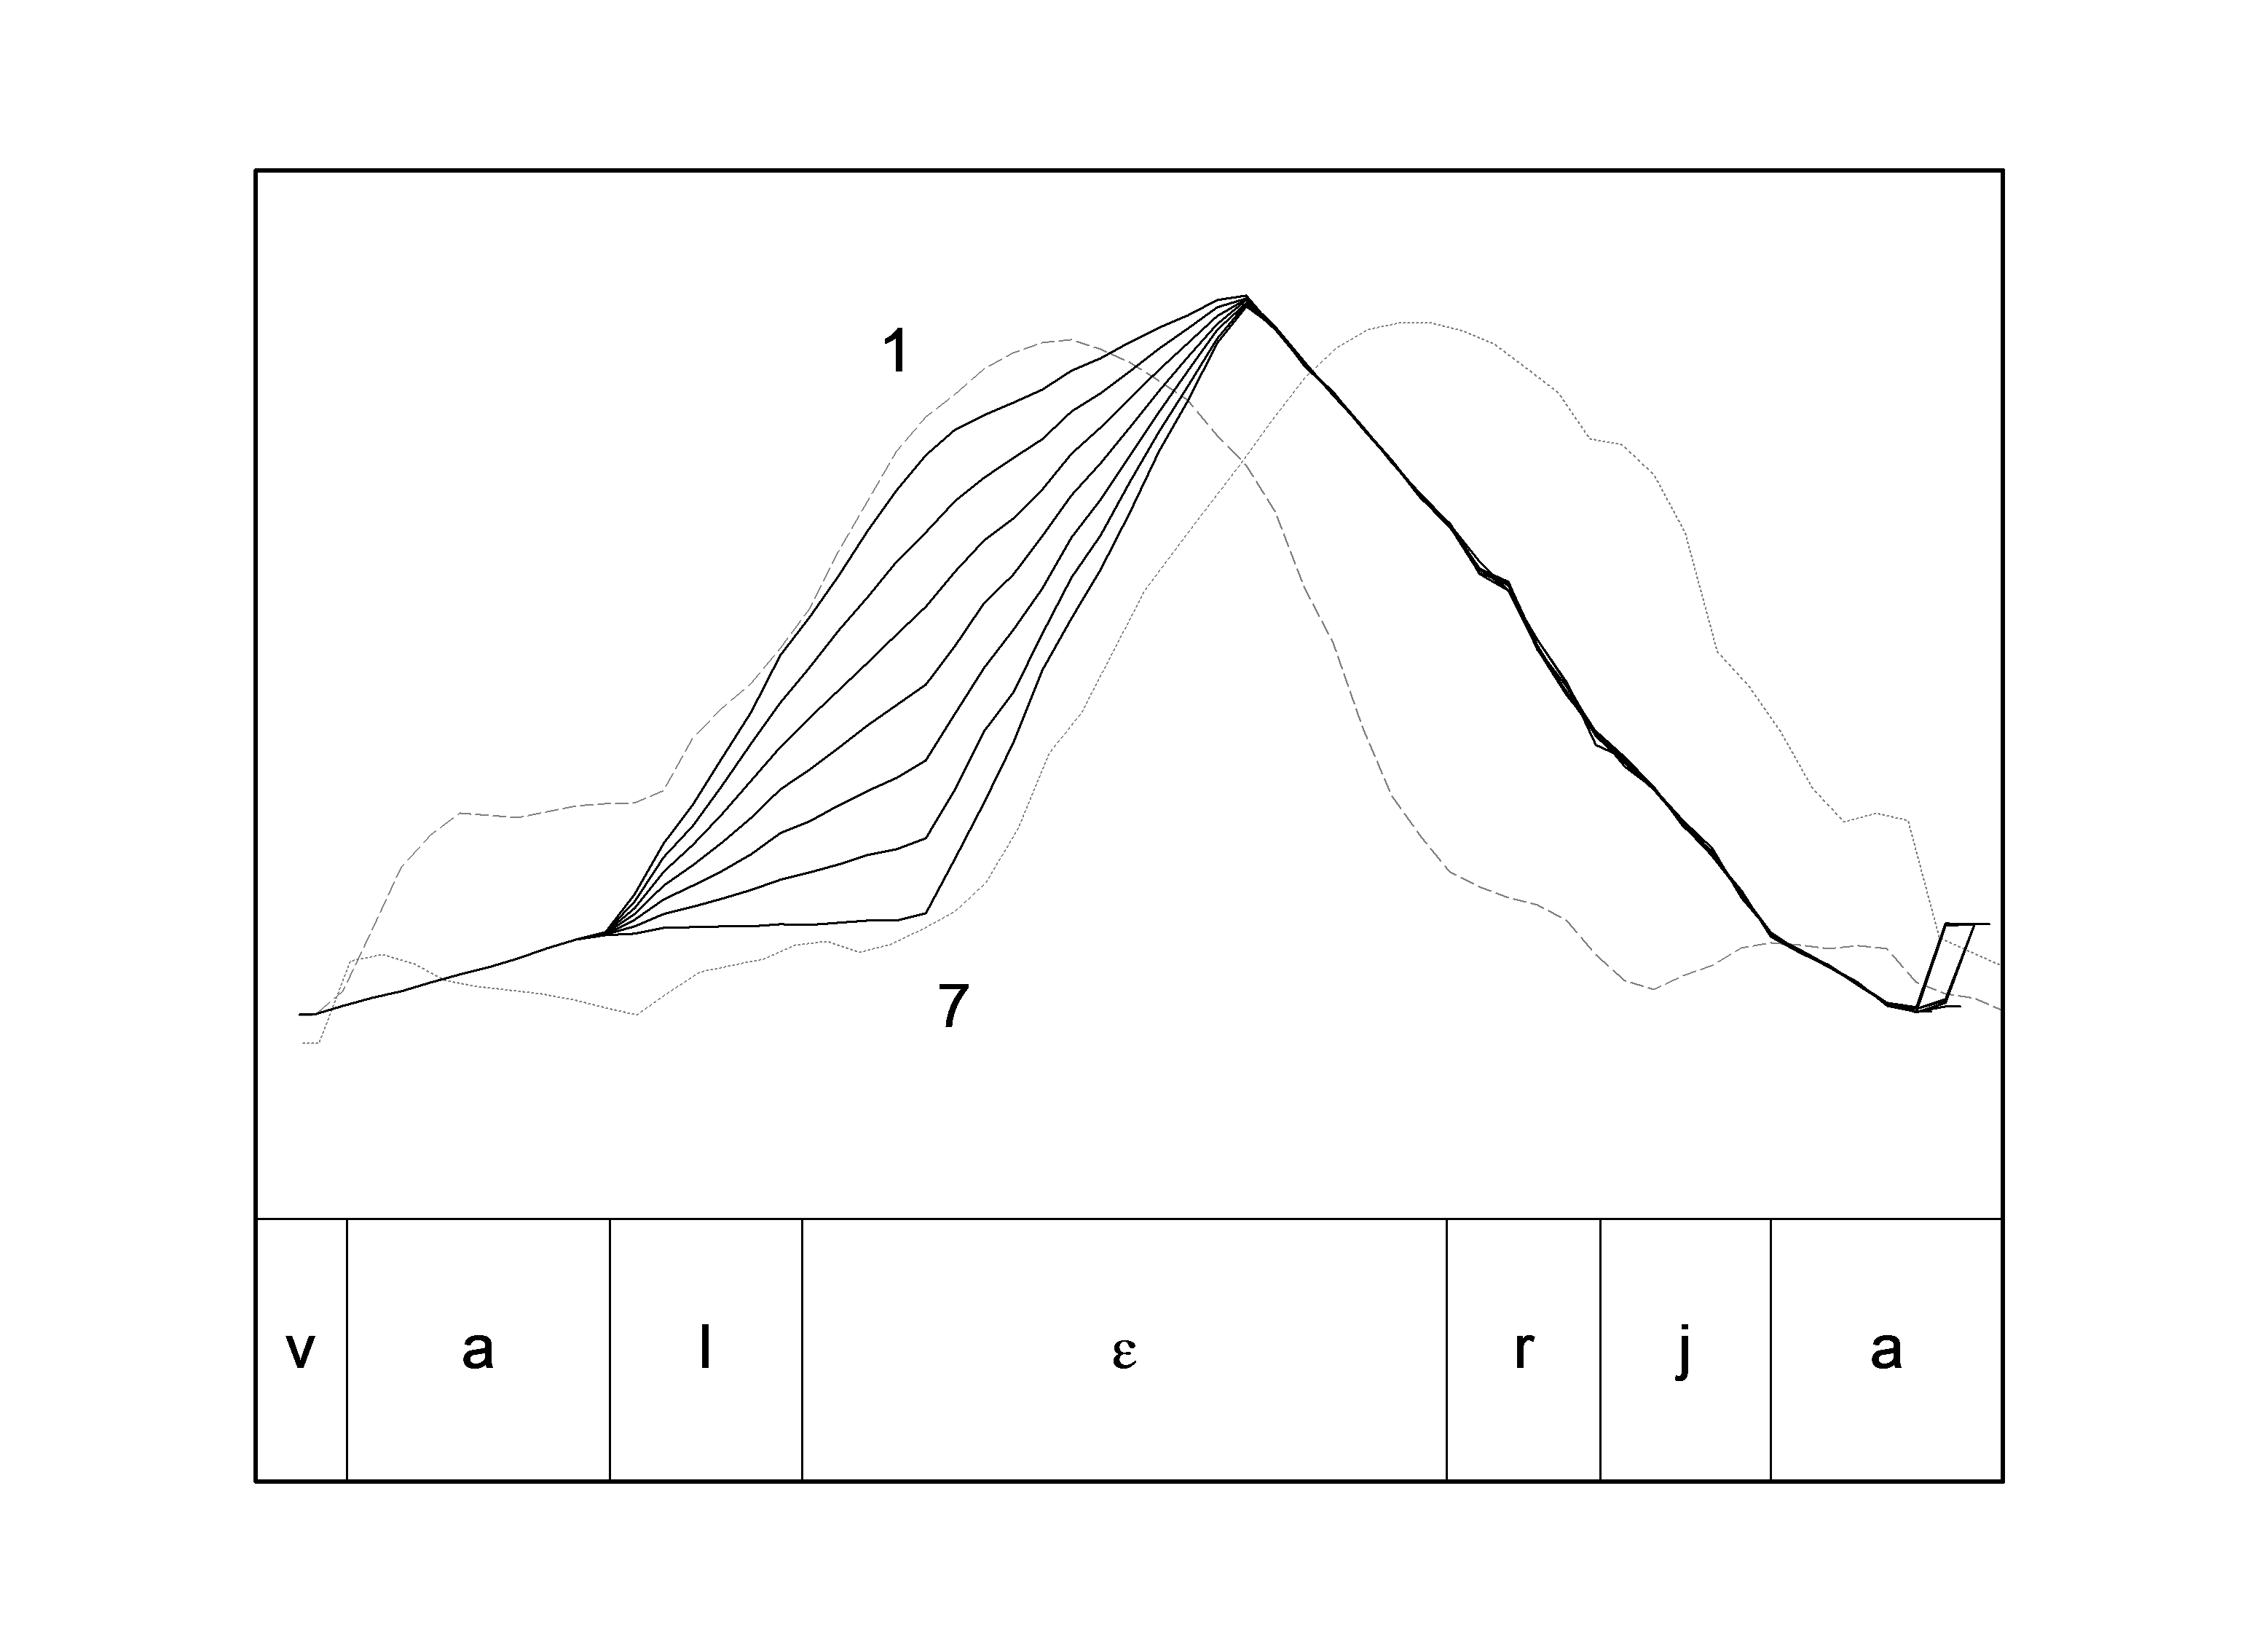
\includegraphics{images/306.png}}
\caption{\textit{f0} contours and averaged phone segmentation for original stimuli (dashed: statement; dotted: question) and resynthezied items (numbers indicate continuum's ends).}
\label{fig306}\end{figure}

We gathered responses for 1050 experimental items (15 subjects x 5 blocks x 7 steps x 2 base stimuli) and 2550 control items (15 subjects x 5 blocks, each composed by 2 base stimuli and 2 repetitions of 16 natural stimuli).

\subsection{Results}\label{sec332}
Responses to control stimuli show that listeners found this task far easier than the preceding one. We had 170 control stimuli for each subject (5 blocks x (2 base stimuli + 2 repetitions x 16 natural stimuli)), and this time only one speaker out of 15 did not reach the 60\% correct response threshold (compare with 17 out of 22 for E1). 

The top panel of Figure~\ref{fig307} shows the observed responses to experimental stimuli. Percent of question responses (y-axis) is plotted against step in manipulation (x-axis, 1 being the most concave and 7 the most convex) separately for items created from the two base stimuli (solid line: question, dashed line: statement). Results show a trend to more question responses for more convex rises. Observed responses to experimental stimuli were fitted to a Logit Mixed Model, in which \textit{Stimulus step} (1 to 7) and \textit{Base stimulus} (Statement or Question) were chosen as fixed factors, while \textit{Subjects} was assigned random status (with variable slope and intercept). Results of the model are shown in Figure~\ref{fig307}, bottom panel.

\begin{figure}
\centering
\resizebox{0.9\linewidth}{!}{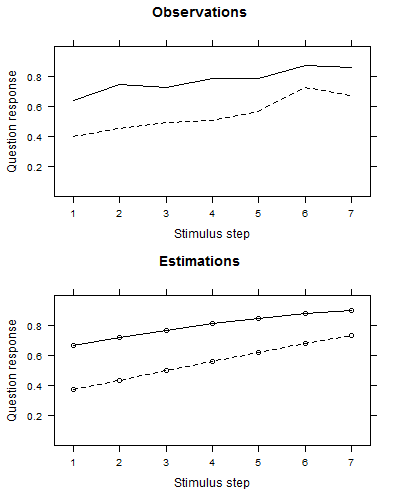
\includegraphics{images/307.png}}
\caption{Experiment II. Observed (top panel) and estimated (bottom panel) question response frequency (y-axis) as a function of manipulation step (x-axis, 1 being very concave and 7 being very convex) and grouped according to base stimulus (solid line: question; dashed line: statement).}
\label{fig307}\end{figure}

\textit{Stimulus step} and \textit{Base stimulus} proved highly significant (respectively, beta= 0.252,  z=3.1, p $<$ 0.002 and beta= -1.196, z=-3.3, p $<$ 0.001), while the interaction between the two factors was not significant (z= -0.018, p= 0.98), indicating that the slopes relative to the two base stimuli are not significantly different. 

This means that, although a Stimulus step effect can be recovered for both continua, items obtain consistently different scores according to the base stimulus from which they are resynthetized. As Figure~\ref{fig307} (right panel) shows, the Question-based stimuli always elicited more Question responses than the respective Statement-based stimuli. Moreover, if for S-based stimuli there is an actual shift in perception,\footnote{From less than 40\% Q-responses for step 1 to more than 60\% Q-responses for step 7, through about 50\% Q-responses for the intermediate step 4.} Q-based stimuli only display a strengthening of Q-responses.\footnote{From more than 60\% for step 1 to more than 90\% for step 7.}

\subsection{Discussion}\label{sec333}
Results from E2 suggest that NI listeners do use rise shape information in order to classify stimuli with ambiguous peak alignment as either questions or statements. Lower rise midpoints (i.e. convex rises) cue more question responses while higher rise midpoints (i.e. concave rises) cue more statement responses, independently of the nature of the stimulus used as starting point for the resynthesis.

As the results for control items show, subjects found the task involving QNF and SNF far easier than the one involving QNF and SPT. 14 subjects out of 15 had a correct classification rate on control stimuli of above 60\%, indicating that judgements on trisyllabic stimuli are reliable. This shows that the low performances recorded for E1 are indeed due to the specific pragmatic contrast under examination, rather than to the task itself (see Section~\ref{sec323}), even if it is reasonable to assume that the rescaling of first name proportions also had a positive effect on listeners' attention (see Section~\ref{sec331}).

Performance rates on control stimuli show that task results are reliable, but the magnitude of the shift in subjects' responses to experimental stimuli indicate that rise shape is not a primary cue.\is{f0 dynamics} While resynthesis of peak alignment can yield up to a 90\% shift in subjects' responses to a question-statement classification task \citep[§3, among others]{dimperio2000role}, in our experiment the shift is only around 30\%. This is consistent with the role of shape information as prosodic detail: in normal conditions, listeners would rely on peak alignment information.\is{prosodic detail} When this information is removed (through averaging in resynthesis), subsidiary information from rise shape can partially surrogate the disambiguation load.

Our results also show that the nature of the base stimulus has a significant effect on subjects' responses. Items resynthesized from a question or statement base always elicited more question or statement responses, respectively. We could speculate that the procedure employed to de-characterize base stimuli (see Section~\ref{sec321}) did not really produce ambiguous items, since it only involved averaging tone scaling and peak alignment. In more general terms, the procedure only involved \textit{f0} manipulations, but we cannot exclude that modality contrasts could also be signalled by cues other than \textit{f0}, such as spectral or rhythmic cues \citep[§5, among others]{niebuhr2010pitchaccent,dimperio2000role}. In the perspective of research on prosodic detail, this finding is particularly interesting: phonological representations of intonation could be underspecified not only with respect to details of phonetic information relative to the fundamental frequency, but also with respect to other prosodic cues.

\section{General discussion}\label{sec34}
The two experiments reported in this chapter aimed at evaluating the perceptual role of shape differences in rising nuclear accents, in order to determine whether the phonological representation of pitch accents must be enriched with dynamic \textit{f0} information. In summary, we could say that E1 and E2 bring mixed evidence to our research question, but they also point towards its broadening. 

In the first experiment we asked our listeners to classify short manipulated stimuli as QNF or SPT. Manipulations were carried out according to the production evidence found in Section~\ref{sec2} (where rises were more convex in Questions and more concave in Statements), under the hypothesis that regularities in production are exploited in perception. The results show that classification is not affected by rise shape manipulation, thus invalidating our research hypothesis. However, the results could have been affected by a number of factors linked to the nature of the task itself, rather than actually mirroring a total lack of significant effects. We devised a follow-up experiment (E2) in order to reduce the impact of some of these possibly confounding factors. Of course, handling negative results is an epistemologically very complex operation, and more than one repair strategy was available. In the following, we discuss three of the improvements we did not apply to E2 (Section~\ref{sec341}; see Section~\ref{sec331} for a discussion of the adopted ones). Then we turn to the main finding of E2, namely the influence of base stimulus category on subjects' responses, and discuss how it reshapes the research question we tackled so far (Section~\ref{sec342}).

\subsection{Possible task improvements}\label{sec341}
To begin with, a first remark is that shape differences cannot be used in classification if they are not perceived at all. That is, if negative results to the classification task proposed in E1 had been complemented by negative results for a parallel discrimination task, dismissing the hypothesis of the perceptual relevance of shape differences would have been easier. We thus proceeded to an informal evaluation of the discriminability of pitch accents with different rise shapes. Given the limited pool of available subjects for this additional task and the encouraging results of the informal exploration (in which three out of three listeners reported to ``hear a difference'' between concave and convex rises), we decided to concentrate our efforts in devising a second classification task. The epistemological assumption behind this choice was that positive results to a second task could have allowed us for a clearer interpretation of the negative results to the first.

Another possible improvement could have been the use of a different task. We have seen in the introduction that identification is not the only task available to the researcher: indeed, semantic differential and context matching have both been already used for the exploration of the perceptual role of prosodic detail. When discussing the results from E1, we stated that one of the possible confounding factor was the use of the labels \textit{Question} and \textit{Answer} for the classification of narrow focus questions and partial topic statements. Given the particularly open pragmatic value of SPT, it is possible that the two labels would not represent equally well the two categories. In E2, we overrode this issue by using narrow focus statements instead of SPT, thus resetting the symmetry between categories and labels. However, it could be noted that the use of a context matching task would have eluded the categories and label issue from its very roots. Upon listening to the excerpted short stimuli, subjects could have been asked to either choose the most appropriate completion between the ones typed on screen, or to rate the appropriateness of one single completion. We could also have avoided the use of possibly misleading labels through the use of a semantic differential task. However, which semantic scales would have allowed us for a clear characterization of QNF and SPT? As we said above, SPT share with Q(NF) a certain degree of openness, in that they qualify as both giving information and suggesting that more information is needed. This feature could have complicated the positioning of SPT on the other hand of QNF on any given semantic scale. For these reasons, we decided to drop the SPT context altogether, in favour of a more straightforward pragmatic contrast. This obviously introduced an asymmetry between the exploration of production and perception data on two different contrasts (production of SPT vs QNF in Section~\ref{sec2}; perception of SNF vs QNF in Section~\ref{sec3}, E2). However, this choice also had the advantage of situating our experiment in the broader frame of other studies on phonetic detail along contrasts in sentence modality, as the work on prenuclear falls in both NI and Northern Standard German we discussed in the introduction (Section~\ref{sec311}).

One last possible improvement to the task was the use of stimuli modified in order to maximize listeners' attention to the possibly relevant cues under investigation. The use of degraded stimuli, for example, has proven useful in the exploration of the role of phonetic detail in talker recognition \citep{sheffert2002learning}. However, as responses to control items in E1 show, no further complexification of task or stimuli was possible, since the subjects already reported serious difficulties in performing the original task, even with simply excerpted (and thus not resynthesized) stimuli.

While the choice of not using degraded stimuli or a semantic differential task was motivated by the reasons we exposed above, the options of a discrimination task or of a context matching had no clear drawbacks, and were discarded only out of the relative unavailability of NI native speakers at the Université de Provence. 

\subsection{A broader research question}\label{sec342}
The perceptual evaluation of shape differences in nuclear rises was instrumental in deciding whether phonological representations of pitch accents should be enriched with dynamic melodic information. The experiments reported in this chapter bring mixed evidence to this research question. On the one hand, the shape differences attested in the SPT vs QNF contrast in production were not found to be used in perception. On the other hand, we documented an effect of rise shape on classification in the SNF vs QNF contrast, a contrast for which we had not documented shape differences in production yet. Perhaps the most linear way to complement our positive perception results was to verify the presence of rise shape differences in production for SNF vs QNF as well. However, we felt that E2 yielded evidence for a phenomenon which could reshape our initial research question altogether: if listeners responses are biased by the nature of the base stimulus even when \textit{f0} contours are made the same (see the offset between the two curves in Figure~\ref{fig307}), then phonological categories could need an enrichment not only with respect to melodic information, but also to phonetic information along different dimensions, such as intensity, duration, voice quality or spectral composition. 

Research on intonational phonology has long acknowledged that cues other than \textit{f0} could play a role in the signalling of post-lexical meaning \citep{hirschberg1992influence}: base-related effects have been reported in perceptual experiments since \citet{dimperio2000role}, and have recently made the object of direct investigation \citep{niebuhr2010pitchaccent}. If other phonetic cues are involved in coding and decoding prosodic categories, the question of whether phonological representations of pitch accents should include dynamic \textit{f0} detail could be generalized and reshaped as to ask whether phonological approaches to intonation should include non-\textit{f0} information. That is, investigating prosodic detail would mean not only to concentrate on unacknowledged features (such as shape) for acknowledged dimension (\textit{f0}), but to unacknowledged features themselves. In the rest of this book we will indeed verify the potential importance of one of such dimensions (namely tempo); the discussion of whether the shape differences we focussed on in this chapter should be accommodated into phonological descriptions of intonation will be necessarily postponed. If duration or intensity variations have to be included in the representation of pitch accents, the restructuring will be deeper than if only new features for already existing dimensions had to be added. For this reason, before suggesting any account of if and how shape differences should be included in phonological representations of pitch accents, we will turn to the potential role of other prosodic cues as prosodic detail.

\section{Conclusion}\label{sec35}
In this chapter we evaluated the perceptual role of rise shape as documented for production in Section~\ref{sec2}. Two experiments based on identification tasks showed that listeners perceive the difference between concave and convex nuclear rises, and that they exploit it for classification purposes. While the first experiment failed to show that classification of Partial Topic Statements and Narrow Focus Questions is affected by rise shape, evidence from the second experiment shows that these negative results might be due to task-related issues. This is because when stimuli are made ambiguous with respect to the main cue of peak alignment, listeners do use rise shape information in order to classify them as Narrow Focus Questions or Statements. 

While not being explicitly tested, a strong effect of the nature of the stimulus used as base for \textit{f0} manipulations was also found in both experiments. In the first experiment, where we only used stimuli resynthesized from a (Partial Topic) Statement base, the listeners who showed the best performance on control stimuli showed a consistent Statement bias for test items. In the second experiment we decided to resynthesize test stimuli from both (Narrow Focus) Question and Statements. Responses from all subjects displayed a strong base effect: for a given step on the continuum in the manipulation of shape proprieties, stimuli resynthesized from a base question always elicited more question responses. That is, while looking for evidence for phonetic detail within a single prosodic dimension (rise shape within \textit{f0} contours), we found reason to believe that other entire prosodic dimensions (duration, intensity, voice quality, spectral proprieties) could represent a source for phonetic detail as well.

Given the possibility of a radical restructuring of phonological representations for pitch accents due to the inclusion of new prosodic dimensions in intonational phonology, our investigation of the role of dynamic melodic detail risks to qualify as minimalist and inconclusive. For these reasons, before returning to the issue of the enrichment of phonological categories, in the next experimental chapters we turn to the evaluation of the role of one of these possible additional dimension, namely tempo, both from a production (Section~\ref{sec4}) and a perception (Section~\ref{sec5}) viewpoint.